\chapter{自然数} \label{chap:natural-number}

自然数集 $\mathbb{N}$ 是我们接触最早的数集,但就是这样一个“性质简单”的数集,我们也能从中发现一些有趣的东西.

\section{认识自然数} \label{sec:understand-natural-number}

自我们出生就一直和数字打交道:人有几根手指?河里有几只鸭子?朴素的我们掰着手指记数:0、1、2、3……10,至此我们会使用 0 到 10 的数字来计数了.

好像有什么不对劲,0 是自然数吗?

不同的书籍、领域给出的答案是不一样的,就根据 \href{https://zh.wikipedia.org/wiki/\%E7\%9A\%AE\%E4\%BA\%9A\%E8\%AF\%BA\%E5\%85\%AC\%E7\%90\%86}{皮亚诺公理} 得出的结论,答案是肯定的.

这五条公理的内容如下:

\begin{enumerate}
  \item 0 是自然数.
  \item 每个自然数 $a$ 有且仅有一个后继数 $a'$ 为自然数.
  \item 对自然数 $b$、$c$,当且仅当 $b' = c'$ 时有 $b = c$.
  \item 0 不是任何自然数的后继数.
  \item 任意有关自然数的命题,若其对自然数 0 成立,且假定它对自然数 $a$ 为真时,可证其对 $a'$ 也成立,那么命题对所有自然数成立.
\end{enumerate}

个人认为把 0 认作自然数的好:离散数学中有单位元(幺元)的概念,若 $0 \notin \mathbb{N}$,则定义在集合 $\mathbb{N}$ 上的二元运算 $+$ 就没有单位元了,让其失去这样的性质就失去了数学的美感.

为了避免 $\mathbb{N}$ 的歧义,我们将尽可能使用 $\mathbb{N}_0$ 表示包含 0 的自然数集,而 $\mathbb{N}^*$ 则表示不包含 0 的自然数集. 当使用 $\mathbb{N}$ 时,默认是包含 0 的自然数集.

\section{四则运算} \label{sec:four-arithmetic-operations}

\subsection{加法} \label{subsec:addition}

\subsection{减法} \label{subsec:subtraction}

\begin{question}
  证明关于 $x_1, x_2, \cdots, x_n$ 的方程组
  \[
    \left\{
    \begin{gathered}
      \prod_{k = 1}^{n} (x_k - \lambda_1) = \mu_1 \\
      \prod_{k = 1}^{n} (x_k - \lambda_2) = \mu_2 \\
      \cdots                                      \\
      \prod_{k = 1}^{n} (x_k - \lambda_n) = \mu_n
    \end{gathered}
    \right.
  \]
  有且仅有确定的解.
\end{question}

\begin{solution}
  设 $f(x) = \prod_{k = 1}^{n} (x - \lambda_k)$,则 $f(x)$ 为 $n$ 次多项式,且其系数为 $\lambda_1, \lambda_2, \cdots, \lambda_n$ 的函数.

  由代数基本定理知 $f(x)$ 有 $n$ 个根,且这些根是 $\lambda_1, \lambda_2, \cdots, \lambda_n$ 的排列.

  故方程组有且仅有确定的解.
\end{solution}

\subsection{乘法} \label{subsec:multiplication}

\subsection{除法} \label{subsec:division}

\subsubsection{取余} \label{subsubsec:modulus}

\section{数的性质} \label{sec:number-properties}

\subsection{负数} \label{subsec:negative-number}

\subsection{奇数} \label{subsec:odd-number}

\subsection{偶数} \label{subsec:even-number}

\subsection{因数} \label{subsec:factor}

\subsection{倍数} \label{subsec:multiple}

\subsection{倒数} \label{subsec:reciprocal}

\subsection{质数} \label{subsec:prime-number}

\subsection{合数} \label{subsec:composite-number}

\section{比较大小} \label{sec:compare-size}

给出自然数 $a$、$b$,现在的我们看到不等式 $a > b$ 时,很容易就得到 $a - b > 0$,未免陷入到了代数的桎梏中——让我们回忆一下我们当初是怎么进行比较的:

\begin{figure}[H]
  \small
  \centering
  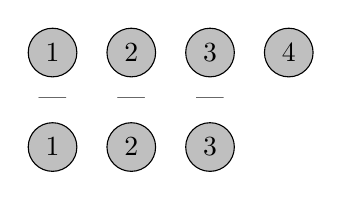
\begin{tikzpicture}
    \foreach \n/\t in
      {0/1,1/2,2/3,3/4}
      {\node[circle,fill=lightgray,draw]
        at (\n,1.2) {$\t$};}

    \foreach \n in
      {0,1,2}
      {\node at (\n,0.6) {|};}

    \foreach \n/\t in
      {0/1,1/2,2/3}
      {\node[circle,fill=lightgray,draw]
        at (\n,0) {$\t$};}
  \end{tikzpicture}
  \caption{比较大小} \label{fig:compare}
\end{figure}

像这样 \strong{一一对应},直到一方比另一方多或相等.

为什么在这讲如此简单的东西呢?我们以一个数学问题切入感受一下:

\begin{question}
  正奇数集 $O = \{1, 3, \cdots\}$ 与正偶数集 $E = \{2, 4, \cdots\}$ 哪个集合的元素个数(势)更大?
\end{question}

\begin{solution}
  存在函数 $f: O \to E, f(x) = x + 1$ 为双射函数,则 $O, E$ 同势.
\end{solution}

而双射的定义如下:

\begin{definition}[双射函数]
  若 $f: X \to Y$ 有 $\forall x \in X$ 存在唯一的 $y$ 与 $x$ 对应,且 $\forall y \in Y$ 存在唯一的 $x$ 与 $y$ 对应,则称 $f$ 为双射函数. 换句话说,如果 $f$ 为两集合间的 \strong{一一对应} 关系,则 $f$ 是双射的.
\end{definition}

在此也请读者们思考:

\begin{problem}[\cref{ans:odd-even-union}] \label{prob:odd-even-union}
$\mathbb{N}^*$ 与 $O, E$ 是否同势?若是请给出函数 $f$,否则给出理由.
\end{problem}

\begin{problem}[\cref{ans:real-number-interval}] \label{prob:real-number-interval}
集合 $A = \{x | 0 < x < 1, x \in \mathbb{R}\}$ 与集合 $\mathbb{R}$ 是否同势?若是请给出函数 $f$,否则给出理由.
\end{problem}

\section{进制} \label{sec:base}

\section{统计} \label{sec:statistics}

\subsection{平均数} \label{subsec:mean}

\subsection{最值} \label{subsec:max-min}

在一组数 $x_1, x_2, \cdots, x_n$ 中,若其中的某个数 $x_k$ 对其中任意一个数 $s$ 有 $x_k \geqslant s$,则称 $x_k$ 为最大值,同理可以给出最小值的定义.

那么根据这样的定义,最大值实际上是可以有“多个”的,比如一下一组数:$0, 1, 1, 2, 2$, 实际上后两个数都是这组数的最大值,只是两者相同而已.

为了避免这样的重复,我们一般将这组数用一个集合表示,而集合中的元素只会出现一次,那么我们搬出严格定义如下:

\begin{definition}[最大元与最小元] \label{def:max-min-element}
  设 $(P,\leqslant )$为偏序集,$S$ 为其子集. 若 $g \in S$ 对任何 $s \in S$ 有 $s \leqslant g$,则 $g$ 称为 $S$ 的 \strong{最大元}(Greatest Element),同理若 $l \in S$ 对任何 $s \in S$ 有 $l \leqslant s$,则 $l$ 称为 $S$ 的 \strong{最小元}(Least Element).
\end{definition}

我们会用多种方式来表示最大值:如 $s_{\max}$、$\max{S}$,在元素个数为二时,我们还可以用一个算式来表达最大值:

记 $M = \max{\{a, b\}}$,则
\begin{equation}
  M = \frac{a + b + |a - b|}{2} \label{eq:max}
\end{equation}

容易证明 $a \geqslant b$ 时 $M = a$,$a < b$ 时 $M = b$.

同理记 $m = \min{\{a, b\}}$,则
\begin{equation}
  m = \frac{a + b - |a - b|}{2} \label{eq:min}
\end{equation}

由此我们就将比较抽象的取最大最小值用准确的算式表达出来了,在未来我们学习随机变量时会利用这个算式的.

\section{坐标} \label{sec:coordinate}

\section{鸡兔同笼} \label{sec:chicken-rabbit}
